%!TEX root = prelim.tex
%!TEX root = fakeroot.tex


\frame{\frametitle{Large Scale Multi PIE experiments}
\begin{center}
\begin{tabular}{|l|c|c|c|c|}
\hline
Rec. Rates & Session 2 & Session 3 & Session 4  \\
\hline
\hline
LDA$_d$ (LDA$_m$) & 5.1 (49.4)\%  & 5.9 (44.3)\% & 4.3 (47.9)\%  \\
\hline
NN$_d$ (NN$_m$)  & 26.4 (67.3)\% & 24.7 (66.2)\% & 21.9 (62.8)\%  \\
\hline
NS$_d$ (NS$_m$) &  30.8 (77.6)\% & 29.4 (74.3)\% & 24.6 (73.4)\% \\
\hline
{Algorithm 1} & {\bf 91.4} \% & {\bf 90.3} \% & {\bf 90.2} \% \\
\hline
\end{tabular}
\end{center}
\begin{columns}
\begin{column}{0.5\textwidth}
\begin{itemize}
{\footnotesize
\item Training: all 249 subj. from session 1\\7 frontal illuminations
\item Testing: all users, from sessions 2-4\\ all 20 illuminations 
\item Use the 88 users not in session 1 for validation
\item Our Algorithm 1 used face detector; no manual intervention
\item subscript m for manual alignment, subscript d for detector
\item neutral expression
}
\end{itemize}
\end{column}
\begin{column}{0.5\textwidth}
\begin{center}
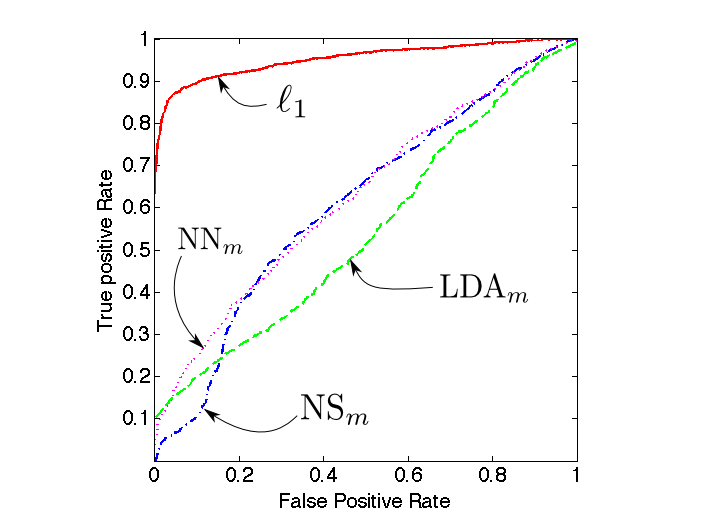
\includegraphics[width=\textwidth]{figures_cvpr/roc3.png}
\end{center}
\end{column}
\end{columns}
}



%%%Cause of errors Our algorithm's errors are mostly caused by a few subjects who significantly change their appearances between sessions (such as hair, facial hair, and eyeglasses). Some representative examples are shown in %Figure \ref{fig:failed-examples}. In fact, for those subjects, alignment and recognition fail on almost all test illuminations.\vspace{0mm} %This may be due the limited number of illuminations present in the training. \vspace{0mm}
%%%\begin{figure}

\renewcommand{\imagesizestring}{width}
\renewcommand{\imagesizea}{0.16\textwidth}
\frame{
\frametitle{Representative examples of failed Multi-PIE subjects}
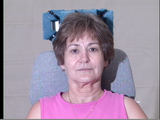
\includegraphics[\imagesizestring =\imagesizea]{figures_cvpr/079_01_01_051_08.png} 
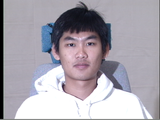
\includegraphics[\imagesizestring =\imagesizea]{figures_cvpr/130_01_01_051_08.png}
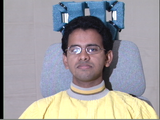
\includegraphics[\imagesizestring =\imagesizea]{figures_cvpr/163_01_01_051_08.png} 
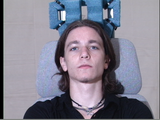
\includegraphics[\imagesizestring =\imagesizea]{figures_cvpr/175_01_01_051_08.png} 
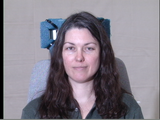
\includegraphics[\imagesizestring =\imagesizea]{figures_cvpr/118_01_01_051_08.png} 
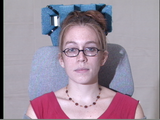
\includegraphics[\imagesizestring =\imagesizea]{figures_cvpr/223_01_01_051_08.png}\\
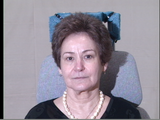
\includegraphics[\imagesizestring =\imagesizea]{figures_cvpr/079_02_01_051_08.png} 
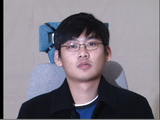
\includegraphics[\imagesizestring =\imagesizea]{figures_cvpr/130_02_01_051_08.png} 
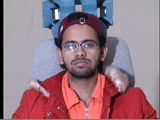
\includegraphics[\imagesizestring =\imagesizea]{figures_cvpr/163_02_01_051_08.png} 
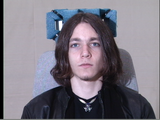
\includegraphics[\imagesizestring =\imagesizea]{figures_cvpr/175_02_01_051_08.png} 
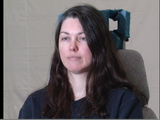
\includegraphics[\imagesizestring =\imagesizea]{figures_cvpr/118_02_01_140_08.png} 
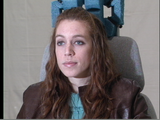
\includegraphics[\imagesizestring =\imagesizea]{figures_cvpr/223_02_01_140_08.png}\\
Trouble when large changes in the appearance between training and testing
\begin{itemize}
\item Hair color, hair style
\item Eyeglasses
\item Facial Hair
\end{itemize}
}

% Experiments on our own training images

\renewcommand{\imagesizestring}{width}
\renewcommand{\imagesizea}{0.2\textwidth}
\frame{\frametitle{Experiments on our data set}
\small{
Training (common to all): 74 users, 38 images per user
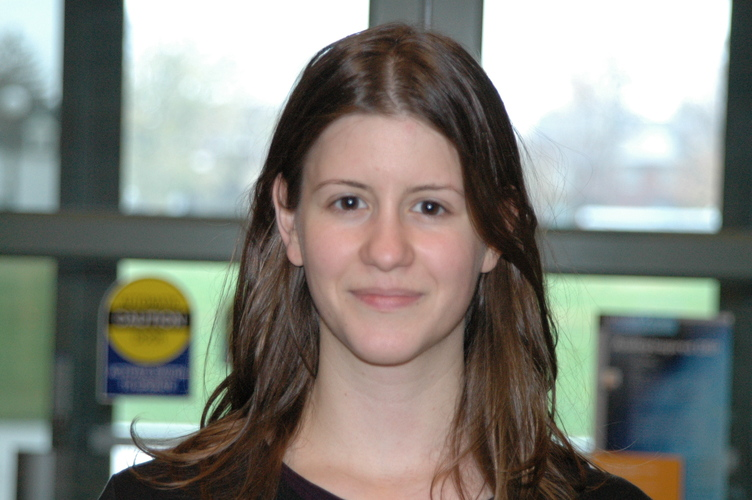
\includegraphics[\imagesizestring =\imagesizea]{figures_cvpr/examples/1/DSC_1319.JPG} 
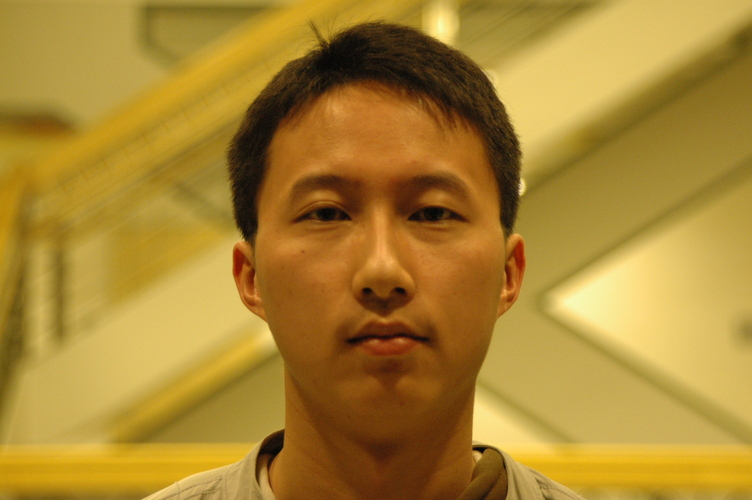
\includegraphics[\imagesizestring =\imagesizea]{figures_cvpr/examples/1/DSC_1531.JPG} 
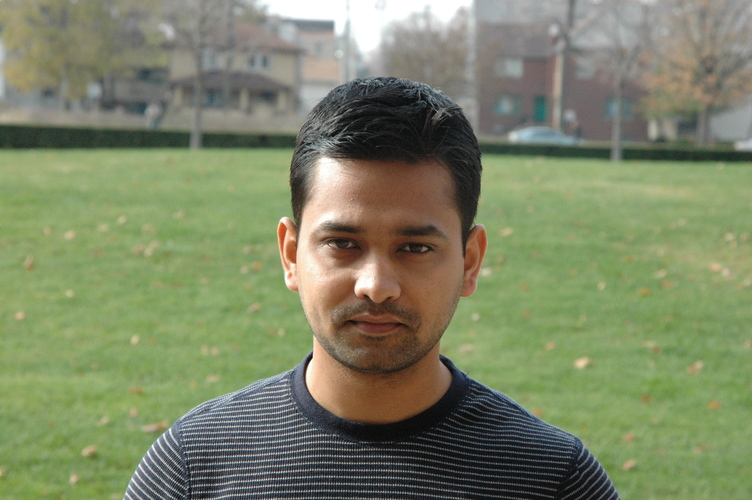
\includegraphics[\imagesizestring =\imagesizea]{figures_cvpr/examples/1/DSC_1574.JPG} 
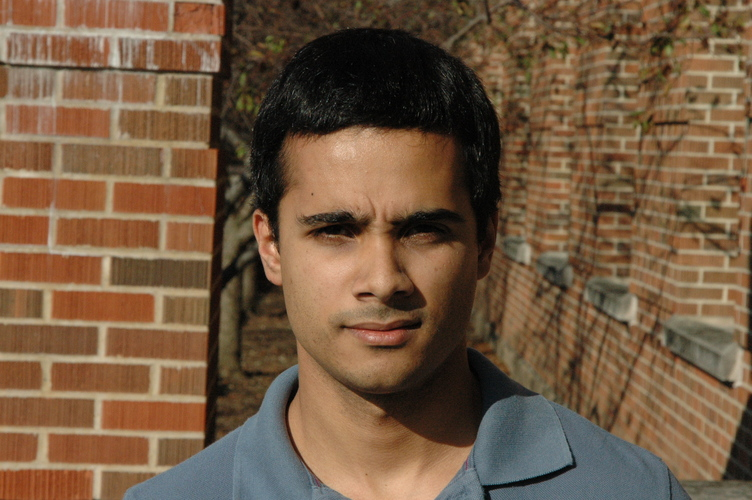
\includegraphics[\imagesizestring =\imagesizea]{figures_cvpr/examples/1/DSC_1622.JPG} 
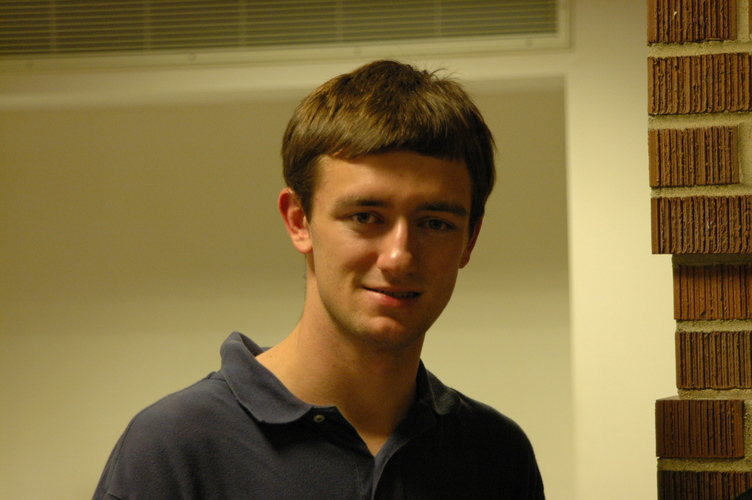
\includegraphics[\imagesizestring =\imagesizea]{figures_cvpr/examples/1/DSC_1786.JPG}\\
Testing: 242 images of 47 subjects, no glasses, frontal view $\Rightarrow \textbf{\color{red} 95.9\%}$ recognition.
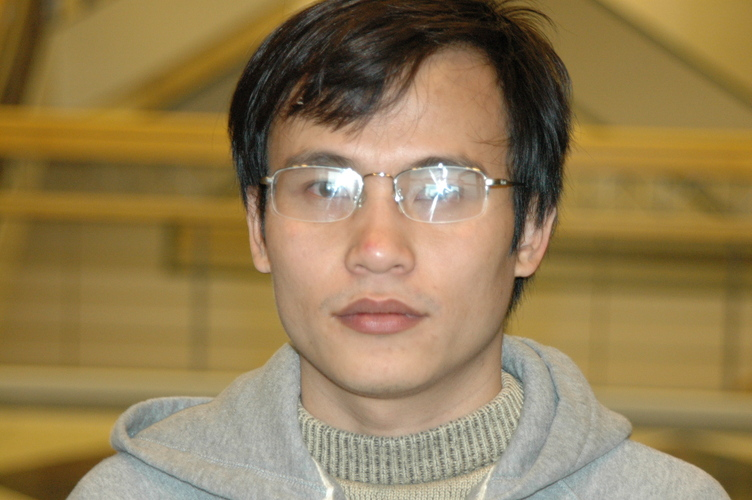
\includegraphics[\imagesizestring =\imagesizea]{figures_cvpr/examples/2/DSC_1448.JPG} 
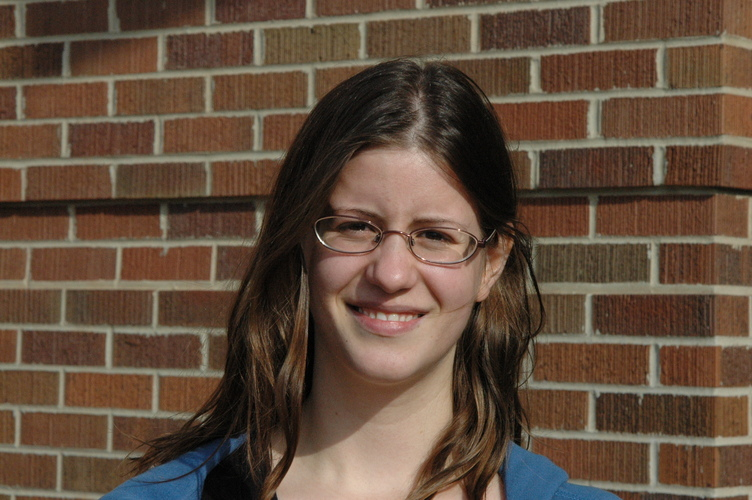
\includegraphics[\imagesizestring =\imagesizea]{figures_cvpr/examples/2/DSC_1585.JPG} 
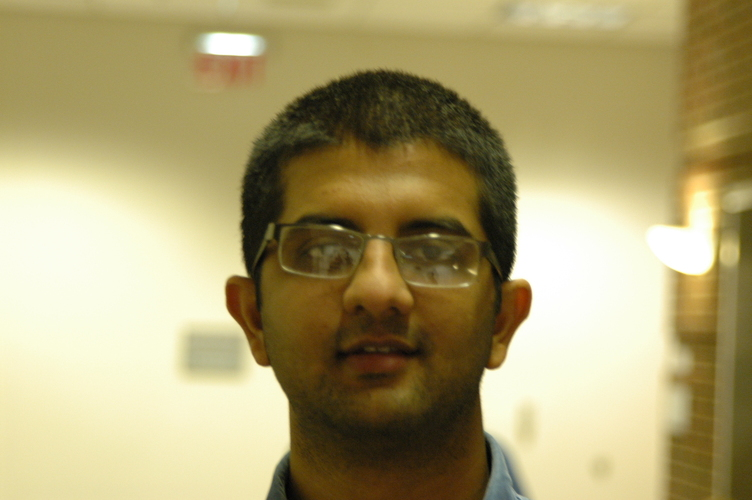
\includegraphics[\imagesizestring =\imagesizea]{figures_cvpr/examples/2/DSC_1588.JPG} 
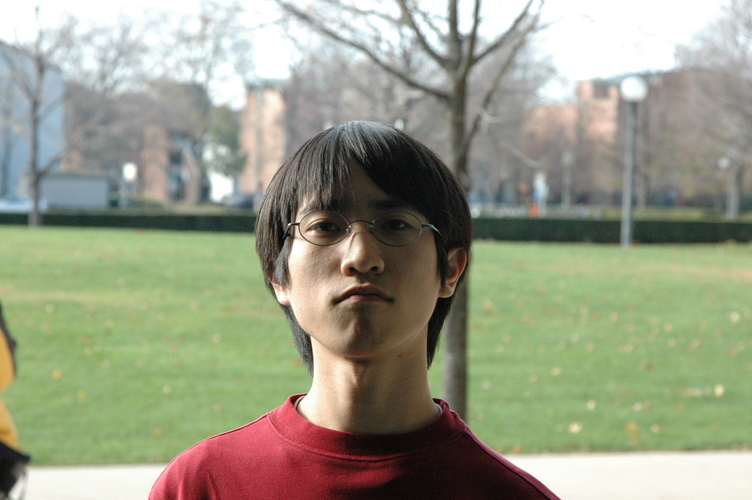
\includegraphics[\imagesizestring =\imagesizea]{figures_cvpr/examples/2/DSC_1666.JPG} 
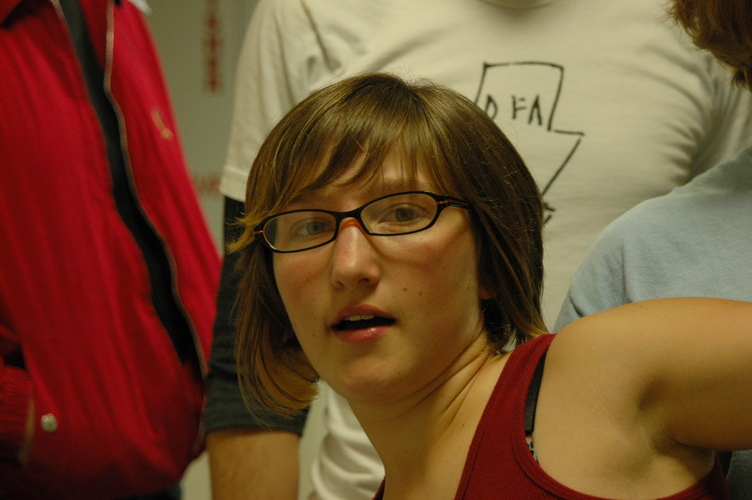
\includegraphics[\imagesizestring =\imagesizea]{figures_cvpr/examples/2/DSC_1874.JPG}\\
Testing: 109 images of 23 subjects with eyeglasses  $\Rightarrow \textbf{\color{red} 91.5\%}$ recognition.
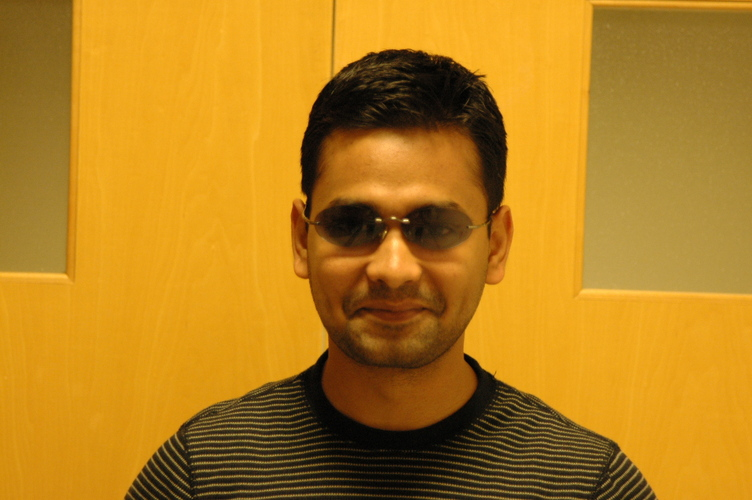
\includegraphics[\imagesizestring =\imagesizea]{figures_cvpr/examples/3/DSC_1572.JPG} 
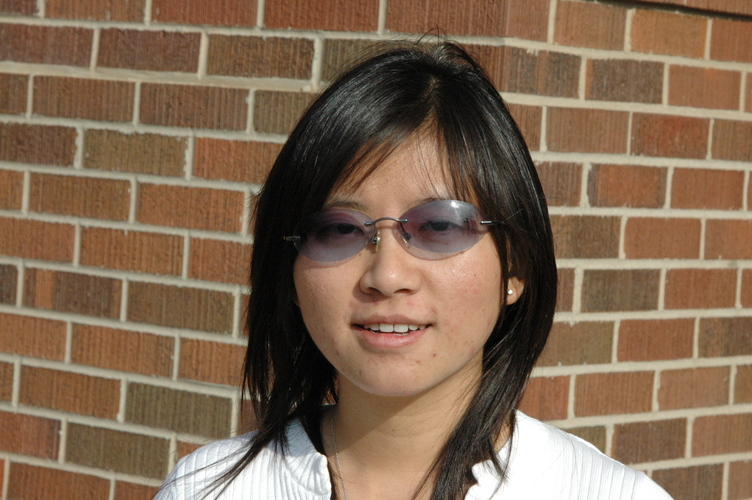
\includegraphics[\imagesizestring =\imagesizea]{figures_cvpr/examples/3/DSC_1587.JPG} 
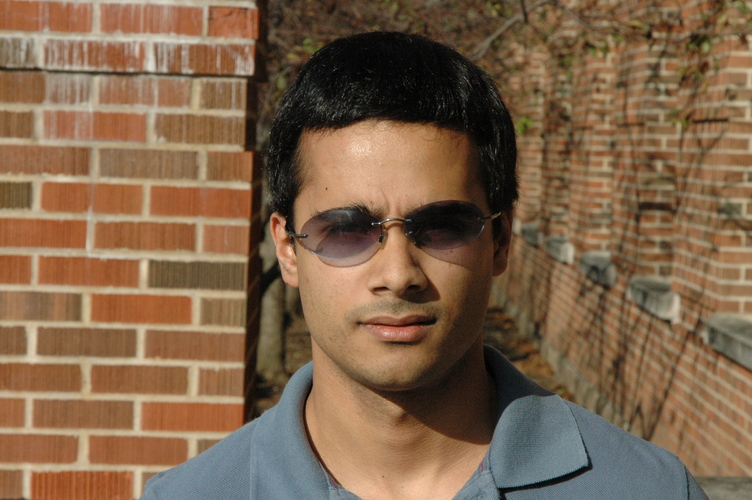
\includegraphics[\imagesizestring =\imagesizea]{figures_cvpr/examples/3/DSC_1623.JPG} 
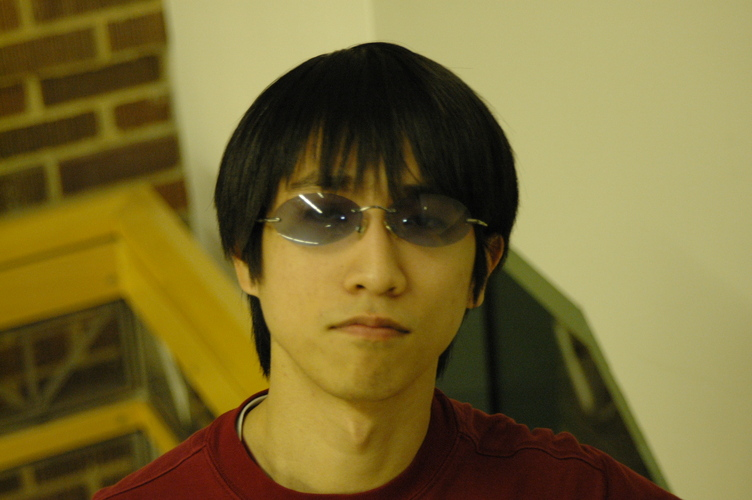
\includegraphics[\imagesizestring =\imagesizea]{figures_cvpr/examples/3/DSC_1652.JPG} 
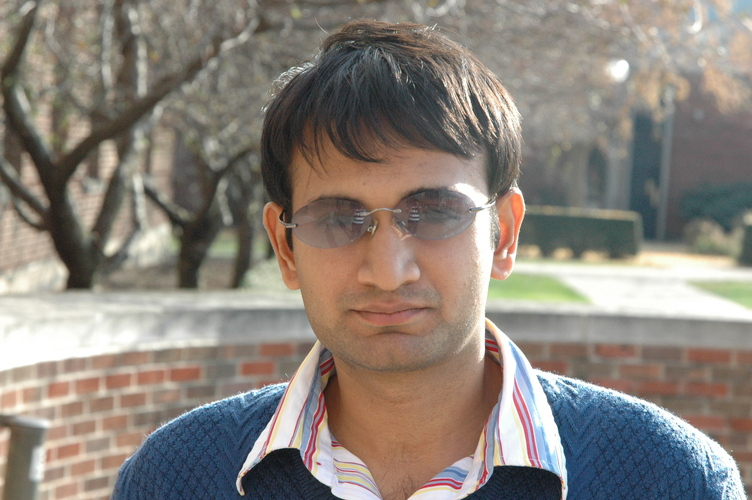
\includegraphics[\imagesizestring =\imagesizea]{figures_cvpr/examples/3/DSC_1675.JPG}\\
Testing: 19 images of 14 subjects with sunglasses $\Rightarrow \textbf{\color{red}63.2\%}$ recognition.
}}



